\section{Thermal-bath effects in quantum quenches}

%\subsection{Kitaev fermionic wires and thermal baths}
\label{modbath}

\subsection{The fermionic Kitaev chain}
\label{kitaevmod}

We consider fermionic Kitaev wires of $L$ sites with open boundary
conditions, whose quantum unitary dynamics is driven by the
Hamiltonian~\cite{Kitaev-2001}
\begin{equation}
  \hat H_{\rm K} = - J \sum_{x=1}^{L-1} \big( \hat c_x^\dagger \hat
  c_{x+1}^{\phantom\dagger} +
  \hat c_x^\dagger \hat c_{x+1}^\dagger+{\rm h.c.}
  \big) - \mu \sum_{x=1}^L \hat n_x ,
  \label{kitaev2}
\end{equation}
where $\hat c_x$ is the fermionic annihilation operator associated
with the site $x$ of the chain, $\hat n_x\equiv \hat
c_x^\dagger \hat c_x^{\phantom\dagger}$ is the particle density
operator.  In the following we assume $J$ as the energy scale, thus we
set $J=1$.

The Hamiltonian~\eqref{kitaev2} can be mapped into a quantum Ising
chain, by means of the Jordan-Wigner transformation, see, e.g.,
Ref.~\cite{S99}.  The corresponding spin model is the
quantum Ising chain with open boundary conditions, i.e.
\begin{equation}
  \hat H_{\rm Is} = -\sum_{x=1}^{L-1} \hat \sigma^{(1)}_x \hat
  \sigma^{(1)}_{x+1} - g\, \sum_{x=1}^L \hat \sigma^{(3)}_x,
  \label{isham}
\end{equation}
$\hat \sigma^{(k)}_x$ being the Pauli matrices and $g=-\mu/2$.  In the
following we prefer to stick with the Kitaev quantum wire, because the
thermal baths and observables that we consider are best defined within
the fermionic model. However, the general scaling scenarios that will
emerge apply to both models.

The Kitaev model undergoes a CQT at $\mu=\mu_c = -2$ (corresponding to
$g=g_c=1$ in the quantum Ising chain), between a disordered quantum
phase for $\mu<\mu_c$ (corresponding to $g>1$) and an ordered quantum
phase for $|\mu|<|\mu_c|$ (corresponding to $|g|<1$). Thus, we define
\begin{equation}
  w = \mu - \mu_c = \mu + 2,
  \label{wdef}
\end{equation}
so that one can easily see the correspondence between the Kitaev
Hamiltonian (\ref{kitaev2}) and the generic one reported in
Eq.~(\ref{hlamt}), i.e. $\hat{H}_c$ corresponds to the Hamiltonian
(\ref{kitaev2}) for $\mu=\mu_c$, and $\hat{H}_p=-\sum_{x=1}^L \hat
n_x$.  The continuous transition at $w=w_c$ belongs to the
two-dimensional Ising universality class~\cite{S99,rossini2021coherent},
characterized by the length-scale critical exponent $\nu=1$, related
to the RG dimension $y_w = 1/\nu=1$ of the Hamiltonian parameter
$w$. This implies that, approaching the critical point, the length
scale $\xi$ of the critical quantum fluctuations diverges as $\xi \sim
|w|^{-\nu}$. The dynamic exponent $z=1$ associated with the unitary
quantum dynamics can be obtained from the power law
$\Delta\sim\xi^{-z}$ of the vanishing gap with increasing $\xi$.
Moreover, the RG dimension of the fermionic operators $\hat c_j$ and
$\hat c^\dagger_j$ at the CQT is $y_c = 1/2$, and that of the particle
density operator $\hat n_x$ is $y_n = 1$~\cite{S99,rossini2021coherent}.


\subsection{Modelization of the thermal bath}
\label{thebath}

In our study we consider a modelization of interaction with a thermal
bath within the Lindblad master equation (\ref{eqlindblad}), whose
asymptotic large-time behavior leads to a Gibbs density matrix at a
given finite temperature $T$. In particular, we consider the proposal
developed in Ref.~\cite{dr2021self} which applies to quantum models
described by quadratic Hamiltonians, such as that of the fermionic
Kitaev wires. This provides a relatively simple modelization of a
thermal bath leading to thermalization in the large-time limit of the
corresponding Lindblad master equation for the density matrix of the
system.

The Kitaev Hamiltonian (\ref{kitaev2}) with open boundary conditions
can be diagonalized in the Nambu field space by a Bogoliubov
transformation, see e.g. Refs.~\cite{PF70,bla86,dr2021self}, so that
we can rewrite it as
\begin{equation}
\hat{H}_{\rm K}=\sum_{k=1}^L\,\omega_k \,\hat b^\dagger_k\, \hat b_k,
  \label{Hdiag}
\end{equation}
where $\omega_k$ are values of the spectrum of the Bogoliubov
eigenoperators $\hat b_k$ (we are neglecting an irrelevant constant
term). Note that both $\omega_k$ and $\hat b_k$ depend on the
Hamiltonian parameter $\mu$.  The relation between the fermionic
operators $\hat{c}_x$ and the Bogoliubov eigenoperators $\hat{b}_k$
can be generally written as~\cite{PF70,bla86,dr2021self}
\begin{equation}
  \label{transBogol}
  \hat c_x = \sum_{k=1}^L A_{xk} \,\hat{b}_k + B_{xk}
  \,\hat{b}_k^\dagger,
\end{equation}
where $A$ and $B$ are appropriate $L\times L$ matrices depending on
$\mu$.  Following Refs.~\cite{dr2021self,CPR-2022-otto_engine}, we write the dissipator
$\mathbb{D}_T[\rho]$ in the Lindblad master equation (\ref{eqlindblad})
in terms of the Bogoliubov eigenoperators as
\begin{eqnarray}
  \mathbb{D}_T[\rho] &=&
\sum_k [1-f(\omega_k,T)]
\left( 2 \,\hat{b}_k\,\rho\,\hat{b}_k^\dagger - 
\{\hat{b}_k^\dagger\hat{b}_k,\rho\}\right)  \nonumber\\
&+&
\sum_k f(\omega_k,T)
\left( 2 \,\hat{b}_k^\dagger\,\rho\,\hat{b}_k - 
\{\hat{b}_k\hat{b}_k^\dagger,\rho\}\right), \label{Dtrho}
\end{eqnarray}
where
\begin{equation}
  f(\omega_k,T) = \left( 1 + e^{\omega_k/T}\right)^{-1}.
  \label{fomt}
\end{equation}
When using this homogeneous dissipator term, the Lindblad master
equation (\ref{eqlindblad}) ensures the asymptotic large-time
thermalization~\cite{dr2021self}. Therefore,
\begin{eqnarray}
  &&\lim_{t\to\infty} \rho(t)  = \rho_t(w,T), \label{asyrho}\\
&&\rho_t(w,T) = \sum_n e^{-E_n(w)/T}|\Phi_n, w\rangle \langle \Phi_n, w|,
 \qquad \label{termrho}
\end{eqnarray}
where $\rho_t(w,T)$ is the density matrix representing the thermal
state, $E_n(w)$ and $|\Phi_n, w\rangle$ are the eigenvalues and
eigenstates of $\hat{H}(w)$.  The asymptotic approach to the thermal
distribution is controlled by the decay-rate parameter
$\gamma$~\cite{dr2021self}. Indeed the Liouvillian gap $\Delta_{\cal L}$
that controls the exponential approach to the asymptotic stationary
state of the Lindblad equation is proportional to the decay rate
$\gamma$, i.e.
\begin{equation}
  \Delta_{\cal L}\sim \gamma.
  \label{deltal}
  \end{equation}

The above modelization of thermal baths provides a useful theoretical
laboratory to investigate issues related to the out-of-equilibrium
dynamics in the presence of thermal baths. Its derivation has
been thoroughly discussed in Ref.~\cite{dr2021self}. We also mention that it
has been employed in Refs.~\cite{CPR-2022-otto_engine,BD-23}.  Some details of the
computations using the Lindblad master equation (\ref{eqlindblad}) with
the dissipator (\ref{Dtrho}) are reported in the appendix.


\subsection{Quantum-quench protocols}
\label{proto}

%As already anticipated in Sec.~\ref{intro}, 
We consider two protocols,
differing for the absence or presence of the contact with the thermal
bath during the quantum evolution after quenching, giving respectively
rise to unitary or dissipative dynamics after quenching. We call them
{\em unitary} and {\em dissipative} QQ protocols, respectively.

\begin{itemize}

\item {\em Unitary} QQ protocol: In this simplest QQ protocol the role
  of the thermal bath is limited to that of preparing the initial
  Gibbs state $\rho_t(w_i,T)$ at $t=0$, reported in
  Eq.~(\ref{eqschrodinger}) with $\rho_0$. This can be obtained by keeping the thermal bath
  in contact with the system for a sufficiently long time $t_{\rm th}$, i.e
  $t_{\rm th}\gg \gamma^{-1}$. Then at $t=0$ the Hamiltonian parameter is
  instantaneously quenched from $w_i<0$ to $w\ge 0$ and the thermal
  bath is removed, so that the subsequent time evolution is that of a
  closed fermionic wire, i.e.  it is unitary and only driven by the
  Hamiltonian of the system.%, cf. Eq.~(\ref{firstprot}).

\item {\em Dissipative} QQ protocol: The quantum evolution starts from
  the same initial Gibbs state $\rho_t(w_i,T)$, but the thermal bath
  is maintained in contact with the system after the QQ from $w_i<0$
  to $w\ge 0$, at $t=0$.  Therefore, the quantum evolution for $t>0$
  is driven by the Lindblad master equation (\ref{eqlindblad}) with the
  dissipator term (\ref{Dtrho}). Note that this dynamic protocol
  entails a further time scale $\tau = \gamma^{-1}$, characterizing
  the asymptotic exponential approach to the large-time stationary
  Gibbs state associated with the Hamiltonian $\hat{H}(w)$ and
  temperature $T$.

\end{itemize}


\subsection{Observables monitoring the time evolution}
\label{obs}


To characterize the dynamic properties of the quantum evolution after
the QQ at $t=0$, we consider the subtracted particle-density average
\begin{eqnarray}
n_s(t,L) = {1\over L} {\rm Tr} \left[ \rho(t) \sum_{x=1}^L \hat{n}_x \right]
- n_c(L),
 \label{ddef}
\end{eqnarray}
 where $n_c(L)$ is the ground-state energy density of the Kitaev wire
 of size $L$ at the critical point $w_c=0$ (in the infinite-size limit
 $n_c= 1/2 - 1/\pi$~\cite{PF70}). Note that the particle density
 operator $\hat{n}_x$ and the transverse spin component
 $\hat\sigma_x^{(3)}$ of the quantum Ising chain (\ref{isham}) are
 trivially related, indeed $\hat{\sigma}_x^{(3)} = 2 \hat{n}_x$.  In
 the definition of $n_s$, the subtraction of $n_c(L)$ simplifies the
 scaling behavior of $n_s(t,L)$ within the critical regime, cancelling
 the leading analytical behavior~\cite{CV2014,rossini2021coherent}. To monitor the
 spatial correlations, we also consider
\begin{eqnarray}
P(x,y,t) & \!\! = \!\! & {\rm Tr}[\rho(t)\,(\hat c_x^\dagger 
\hat c_{y}^\dagger +
    \hat c_{y} \hat c_{x})],\label{ptf}\\ 
C(x,y,t) & \!\! = \!\! & {\rm Tr}[\rho(t)\, (\hat c_x^\dagger \hat c_{y} 
+ \hat
    c_{y}^\dagger \hat c_{x})].\label{gtf} 
\end{eqnarray}

Some details on the computation of the above quantities during the
time evolution of the QQ protocols are reported in the appendix.


\subsection{Out-of-equilibrium scaling}
\label{scabeh}

We now discuss the out-of-equilibrium behaviors arising from the QQ
protocols outlined in Sec.~\ref{proto}.  We show that they develop
OFSS behaviors where the effects of the thermal baths are taken into
account by appropriate extensions of the out-of-equilibrium
zero-temperature scaling laws describing soft QQs in
closed systems within their critical regime, already put foward by
earlier works~\cite{pelissetto2017dynamic,rossini2021coherent}.

\begin{figure}[!htb]
\centering
  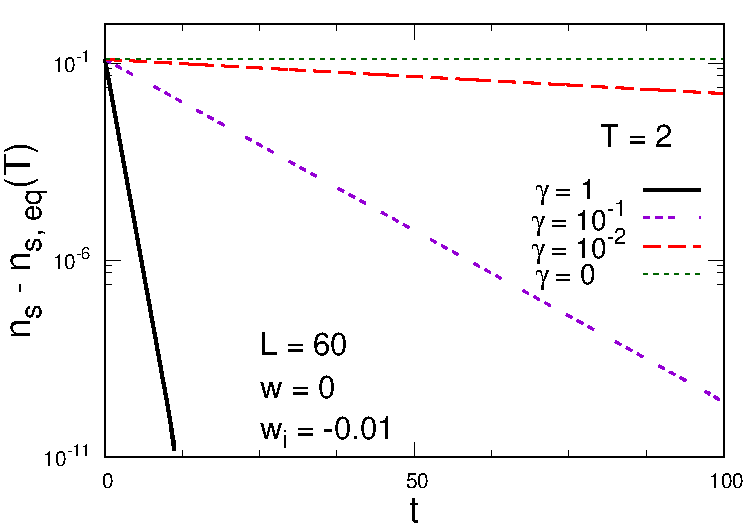
\includegraphics[width=0.6\columnwidth]{imm/NT2l60diffglog.pdf}
  \caption{The quantum evolution of the subtracted particle density
    $n_s(t)$, cf. Eq.~(\ref{ddef}), for the dissipative QQ protocol
    entailing a dissipative dynamics after the QQ at $t=0$ of the
    Hamiltonian parameter $w$, describing the persistent interaction
    with the thermal bath, cf.  Eqs.~(\ref{eqlindblad}) and
    (\ref{Dtrho}).  These curves refer to a system of size $L=60$,
    temperature $T=2$ of the thermal bath, quenching from $w_i=-0.01$
    to $w=0$, and various values of the decay rate $\gamma$ (the case
    $\gamma=0$ corresponds to the evolution of the close system).  We
    plot the difference $n_s(t,L,T) - n_{s,{\rm eq}}(L,T)$ which is
    expected to vanish in the large-time limit.  In this figure and in
    the following ones, the unity that we use are such that
    $\hslash=1$, $k_B=1$, and $J=1$.}
  \label{plainns}
\end{figure}



The OFSS behaviors that we put forward for QQ protocols considered are
verified by numerical computations for the fermionic Kitaev wire up to
relatively large sizes. See the appendix for details on such
calculations.

As a preliminary example of out-of-equilibriun QQ
behaviors that we want to address, in Fig.~\ref{plainns} we show some
results for the quantum evolution of the subtracted particle density
(\ref{ddef}) along the dissipative protocol outlined in
Sec.~\ref{proto}, after quenching a fermionic Kitaev wire of size
$L=60$, from $w_i=-0.01$ to $w=0$, in the presence of a thermal bath
at a temperature $T=2$, and various values of the decay rate $\gamma$.
The quantum evolution turns out to have a significant dependence on
the decay-rate parameter $\gamma$ that characterized the interactions
between the system and the thermal bath. Indeed, the curves of the
substracted particle density appear to approach its equilibrium value
$n_{s,{\rm eq}}(w=0,T=2)\approx 0.0004601...$ (while at $t=0$ we have
$n_{s,{\rm eq}}(w=w_i,T=2) \approx 0.126598...$), faster and faster
with increasing $\gamma$, actually exponentially as $\exp(-t/\tau)$
with $\tau\sim\gamma^{-1}$, conferming the role of decay rate of the
parameter $\gamma$ within the Lindblad master equation,
cf. Eq.~(\ref{deltal}). Analogous results are obtained for other
observables, such as fermionic correlation functions defined in
Sec.~\ref{obs}. In the following we put forward an out-of-equilibrium
scaling theory for these out-of-equilibrium phenomena within the
quantum critical regime.




\subsubsection{Zero-temperature scaling in quantum quenches}
\label{zeroT}

We now provide a brief summary of the out-of-equilibrium scaling
theory for close systems, describing QQ protocols within the critical
regime~\cite{pelissetto2017dynamic,rossini2021coherent}. The initial state is the ground state
associated with an initial value $w_i<0$, and, after the instantaneous
quench at $t=0$ from $w_i$ to $w$, the quantum evolution is driven by
the Schr\"odinger equation.

Out-of-equilibrium scaling laws can be obtained by extending those
valid at equilibrium, allowing for a time dependence essentially
controlled by the time scaling variable $\Theta \sim t\,\Delta$, which
is obtained by assuming that the relevant time scale of the critical
modes is proportional to the inverse energy difference $\Delta$ of the
lowest states. We refer to Ref.~\cite{rossini2021coherent} for a through
presentation of the scaling arguments leading to the asymptotic OFSS
behaviors.

Let us consider the out-of-equilibrium evolution (after quenching) of
generic observables, such as the expectation value $O$ at time $t$ of
a local operator $\hat{O}({\bm x})$ and its fixed-time correlations
$G_O=\langle \hat{O}({\bm x}) \hat{O}({\bm y})\rangle$. The general
working hypothesis underlying out-of-equilibrium FSS frameworks is
that the expectation value of $\hat{O}({\bm x})$ and its correlation
functions obey asymptotic homogeneous scaling laws~\cite{rossini2021coherent}, such
as
\begin{eqnarray}
O(t, {\bm x}, L, w_i, w) \approx  b^{-y_o} {\cal O}(t/b^z,
{\bm x}/b, L/b, b^{y_w} w_i, b^{y_w} w),\quad
    \label{Oscaquefss0}
\end{eqnarray}
  where $b$ is an arbitrary (large) length scale, $y_o$ is the RG
  dimension of the local operator $\hat{O}_{\bm x}$ and the RG
  exponents $y_w$ and $z$ are determined by the universality class of
  the CQT (they are the RG dimensions of the Hamiltonian parameter $w$
  and the temperature $T$, respectively). Thus both the initial and
  final values of $w$, i.e.  $w_i$ and $w$, take the same RG exponent
  $y_w$, being coupled to the RG perturbation ${\hat H}_p$ within the
  Hamiltonian. Note that we do not assume translation invariance,
  which is generally broken by the presence of boundaries, such as
  those arising from open boundary conditions.
  
 
OFSS can be straightforwardly derived by fixing $b=L$ in the above
homogenous scaling law. Then, we expect the OFSS of the expectation
value $O$ of a generic local operator $\hat{O}_{\bm x}$, of its
spatial average $\hat{O}_a =L^{-d}\sum_{\bm x}\hat{O}_{\bm x}$, and
its two-point correlation function $G_O$, develop the asymptotic OFSS
behavior~\cite{pelissetto2017dynamic,rossini2021coherent}
\begin{eqnarray}
  && O(t, {\bm x}, L, w_i, w) \, \approx \, L^{-y_o} \,
  {\cal O}(\Theta, {\bm X}, \Phi_i, \Phi),
\nonumber\\
  && O_a(t, L, w_i, w) \, \approx \, L^{-y_o} \, {\cal O}_a(\Theta,
\Phi_i, \Phi),   \label{Oscaquefss}\\
  && G_{O}(t, {\bm x}_1, {\bm x}_2, L,
  w_i, w) \, \approx \, L^{-2y_o} \, {\cal G}_{O}(\Theta, {\bm X}_1,
  {\bm X}_2, \Phi_i, \Phi), \nonumber
\end{eqnarray}
where the scaling variables appearing in the scaling functions ${\cal
  O}$, ${\cal O}_a$, and ${\cal G}_O$ are defined as
\begin{equation}
  \Theta\equiv\frac{t}{L^z},\;\; {\bm X}_i \equiv \frac{{\bm x}_i}{L},\;\;
  \Phi_{i} \equiv
L^{y_w} \, w_i , \;\; \Phi \equiv L^{y_w} \,w.
  \label{scalvarque}
\end{equation}
The OFSS limit is obtained in the large-$L$ and large-$t$ limit
keeping the above scaling variables fixed. These conditions ensure
that the system remains within the universal critical regime during
the quantum evolution.  Note that in the scaling law
(\ref{scalvarque}) the dynamic features are essentially encoded in the
time dependence of the scaling variable $\Theta\sim t\,\Delta$.  The
other features, in particular when $w_i=w$, are analogous to those
arising from equilibrium FSS at CQTs~\cite{CV2014,rossini2021coherent}, where the
argument $\Phi=L^{y_w} w$ of the scaling functions is controlled by
the RG dimension $y_w$ of the relevant parameters $w$ at the RG fixed
point associated with the CQT.


The above OFSS equations can be straightforwardly applied to the
observables defined in Sec.~\ref{obs}, after a quench from $w_i$ to
$w$ at $t=0$, keeping into account that the RG dimension of the
subtracted particle density is $y_n = 1$, and that of the fermionic
operator $\hat c_x$ is $y_c=1/2$.  Note that the dominant analytical
contributions to the particle density~\cite{CV2014,rossini2021coherent} coming from
the analytical background are canceled in the difference $n_s$ defined
in Eq.~(\ref{ddef}), whose leading asymptotic behavior arises from the
quantum critical modes, therefore it is analogous to that of $O_a$ in
Eq.~(\ref{Oscaquefss}), with $y_o=y_n$.  Analogously one can apply the
OFSS in Eq.~(\ref{Oscaquefss}) to observables and correlation
functions constructed with the spin operators of the quantum spin
chain (\ref{isham}).  The OFSS functions are expected to be universal
with respect to the microscopic details of the model, apart from
nonuniversal multiplicative rescaling and normalizations of its
arguments.  Within isolated fermionc Kitaev wires and quantum Ising
chains, the OFSS arising from soft QQs has been verified by numerical
computations for various boundary conditions, and also along their
quantum first-order transition line~\cite{pelissetto2017dynamic,rossini2021coherent}.





The OFSS limit is expected to be approached with power-law suppressed
corrections.  There are various sources of scaling corrections when
approaching the OFSS. Of course, they include those that are already
present at equilibrium. In particular, the irrelevant RG perturbations
are sources of scaling corrections for the asymptotic behavior of the
free-energy density~\cite{PV2002,rossini2021coherent}.  In the case of
one-dimensional quantum systems undergoing CQTs belonging to the
two-dimensional Ising universality class, the leading scaling
corrections from irrelevant RG perturbations are suppressed as
$L^{-\omega}$ with $\omega=2$~\cite{CHPV-02,CV2014}. However, other
contributions may become more relevant~\cite{PV2002,CV2014,rossini2021coherent}, such
as those arising from the presence of analytical backgrounds, from the
presence of boundaries (which generally gives rise to $O(1/L)$
corrections), and, in the case of correlation functions, from RG
mixings of the source fields [this for example happens in the case of
  the correlation functions of the fermionic field $\hat{c}_x$, for
  which corrections are $O(1/L)$].  These scaling corrections have
been confirmed by numerical results~\cite{CV2014,rossini2021coherent}. Therefore, we
expect that the asymptotic OFSS of fermionic Kitaev wires and quantum
Ising chains with open boundary conditions is generally approached
with $O(1/L)$ corrections.




\subsubsection{OFSS along the unitary QQ protocol}
\label{scalprota}



For the simplest unitary protocol reported in Sec.~\ref{proto}, where
the quantum evolution is that of the isolated fermionic wire, the
request that the dynamics remains within the critical regime implies
that the temperature of the initial Gibbs state must be appropriately
suppressed in the large-$L$ OFSS limit, to obtain a nontrivial
out-of-equilibrium critical limit.  This is analogous to what happens
within the equilibrium FSS, where one introduces the scaling
variable~\cite{SGCS-97,S99,rossini2021coherent}
\begin{equation}
  \Xi \equiv L^z T,
 \label{Xidef}
\end{equation}
to allow for a nonzero temperature in the FSS of the observables.
Therefore, like equilibrium FSS, we conjecture that the temperature of
the initial Gibbs state enters the OFSS associated with the unitary QQ
protocol by adding a further dependence on $\Xi$ in the scaling
functions (\ref{Oscaquefss}).  In other words, a nontrivial asymptotic
OFSS limit is expected to be realized in the large-$L$ and large-$t$
limits keeping also $\Xi$ fixed, beside the scaling variables already
defined in Eq.~(\ref{scalvarque}).  Therefore, we expect that the OFSS
of standard QQ protocols starting from ground states,
cf. Eq.~(\ref{Oscaquefss}), changes into
\begin{eqnarray}
   O(t, {\bm x}, L, w_i, w, T) \, \approx \, L^{-y_o} \, {\cal
    O}(\Theta, {\bm X}, \Phi_i, \Phi, \Xi),
    \label{Oscaquefssa}
\end{eqnarray}
and analogously for its spatial average $O_a$ and the correlation
function $G_O$.

\begin{figure}[!htb]
\centering
  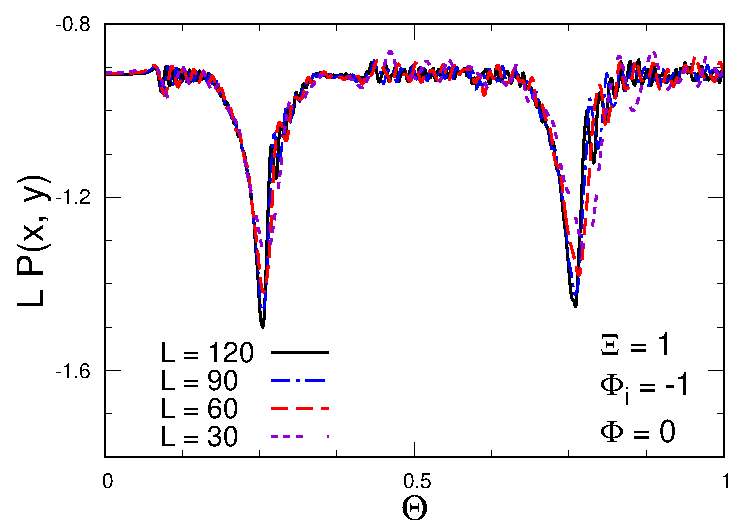
\includegraphics[width=0.6\columnwidth]{imm/LPk-1q0e100g0.pdf}
  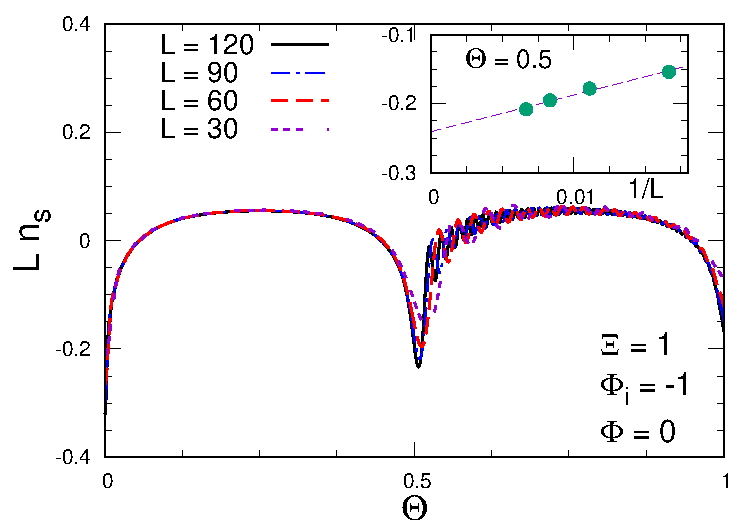
\includegraphics[width=0.6\columnwidth]{imm/LNk-1q0e100g0.pdf}
  \caption{OFSS behavior of the subtracted particle density (bottom)
    and the fermionic correlation function $P(x=L/3,y=2L/3,t)$,
    cf. Eq.~(\ref{ptf}), arising from the unitary QQ protocol, for
    various lattice sizes $L$, at fixed $\Xi=L^z T =1$,
    $\Phi_i=L^{y_w} w_i=-1$ and $\Phi=L^{y_w} w=0$, versus the time
    scaling variable $\Theta=t/L^z$.  These computations nicely
    support the OFSS behaviors reported in
    Eq.~(\ref{Oscaquefssa}). The inset of the bottom figure shows that
    the approach to the OFSS limit is consistent with $O(1/L)$
    corrections.  Analogous results are obtained for other values of
    the scaling variables.}
  \label{protares}
\end{figure}


The numerical analysis for the fermionic Kitaev wire under the unitary
protocol fully support to this OFSS, obtained by extending the QQ FSS
behaviors of closed systems starting from an initial ground
state. This is clearly demonstrated by the curves reported in
Fig.~\ref{protares}, associated with the quantum evolutions of the
subtracted particle density $n_s(t)$ and the fermionic correlation
$P(x,y,t)$ (the other fermionic correlation $C(x,y,t)$ develops an
analogous OFSS).



\subsubsection{OFSS along the dissipative QQ protocol}
\label{scalprotb}

We now discuss the dynamics arising from the dissipative protocol
outlined in Sec.~\ref{proto}, when the quantum evolution after
quenching is described by the Lindblad master equation
(\ref{eqlindblad}) with the thermal-like dissipator (\ref{Dtrho}), to
modelize the interaction with a thermal bath characterized by a
temperature $T$ (which does not change after quenching)
and decay rate $\gamma$.

\begin{figure}[!htb]
\centering
  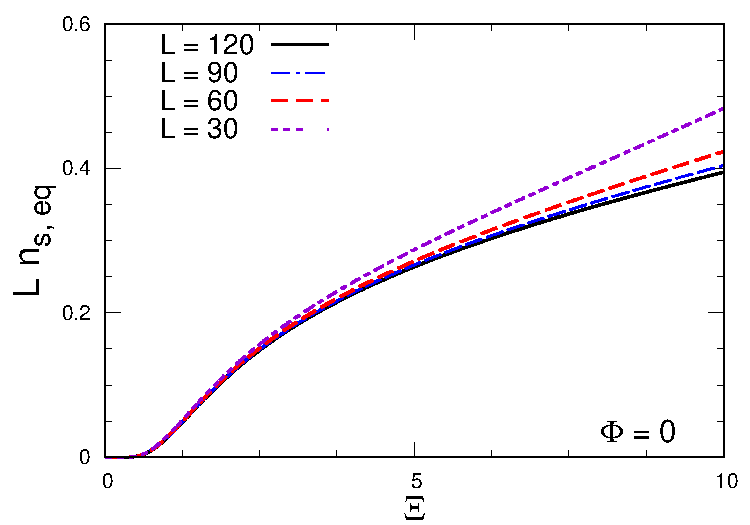
\includegraphics[width=0.6\columnwidth]{imm/LNeqXik0.pdf}
  \caption{ Equilibrium FSS of the subtracted particle density
    $n_{s,{\rm eq}}$ at the critical point $w=0$, versus the rescaled
    temperature $\Xi=L^z T$. With increasing $L$, the data show the
    expected convergence to the equilibrium FSS reported in
    Eq.~(\ref{nseqsca}) with $y_n=1$. }
  \label{eqns}
\end{figure}

  
\begin{figure}[!htb]
\centering
  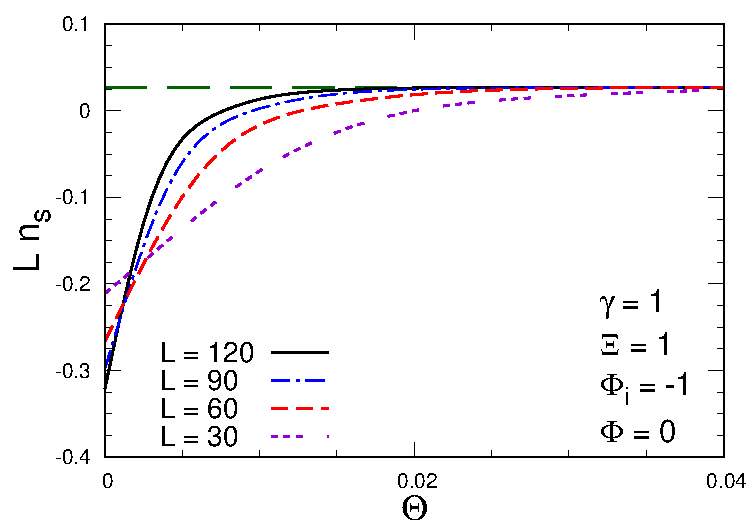
\includegraphics[width=0.6\columnwidth]{imm/LNk-1q0e100t100g1000.pdf}
  \caption{Quantum evolution of the subtracted particle density
    arising from the dissipative QQ protocol, when rescaling all
    quantities involved in the quench protocol, except for the decay
    rate $\gamma$. With increasing $L$, the curves appear to approach
    the equilibrium FSS value at finite temperature (where the
    temperature dependence enters through the scaling variable
    $\Xi=L^z T$) faster and faster, reflecting a nonuniform
    convergence for any $\Theta>0$. The dashed line shows the
    equilibrium value of $n_s$ for $\Phi=0$ and $\Xi=1$, which is
    asymptotically approached by the various curves.  }
  \label{protbresgamma}
\end{figure}



We expect that the temperature $T$ of the thermal bath must be
rescaled as in the case of the unitary QQ protocol, i.e. we must
consider again the associated scaling variable $\Xi$ already defined
in Eq.~(\ref{Xidef}).  However, since the QQ moves the system
out-of-equilibrium, also the decay rate $\gamma$, and corresponding
time scale $\tau=\gamma^{-1}$, associated with the interactions with
the thermal bath is expected to play a relevant role to establish a
corresponding nontrivial OFSS limit.  This was already noted in
Ref.~\cite{BD-23} in the analysis of dynamic protocols entailing the
variation of the temperature at the critical point.

When keeping $\tau$ constant in the FSS limit where the
scaling variable $\Theta=t/L^z$ is kept fixed, in the large-$L$ limit
we have eventually that
\begin{equation}
  t = \Theta \, L^z \gg \tau,
  \label{tggtau}
  \end{equation}
which is the condition ensuring thermalization for any finite value
$\Theta>0$. Therefore, when keeping $\tau$ fixed, the quantum
evolution is not expected to develop a nontrivial OFSS limit. Indeed,
in the large-$L$ limit, the system turns out to suddenly approach an
equilibrium Gibbs state (associated with the Hamiltonian parameter $w$
and temperature $T$) with respect to the rescaled time $\Theta$,
without any further relevant evolution of the system for any
$\Theta>0$.  Therefore, if the temperature is rescaled by keeping
$\Xi=L^z T$ fixed, we must recover the equilibrium FSS behavior in the
presence of a thermal bath at temperature $T$, such as that associated
with the subtracted particle density~\cite{CV2014,rossini2021coherent}
\begin{equation}
  n_{s,{\rm eq}}(w,L,T) \approx L^{-y_n} {\cal N}(\Phi,\Xi),
  \label{nseqsca}
  \end{equation}
where $\Phi=L^{y_w} w$, and the temperature dependence enters through
the associated scaling variable $\Xi=L^z T$.  In Fig.~\ref{eqns} we
show some equilibrium data at the critical point $w=\Phi=0$, versus
$\Xi$, showing the approach to the asymptotic large-$L$ equilibrium
FSS (\ref{nseqsca}).  The realization of the equilibrium FSS within
the QQ protocol at fixed $\gamma$ is demonstrated by the plots
reported in Fig.~\ref{protbresgamma}, which show the somewhat trivial
convergence toward the equilibrium FSS for any finite $\Theta>0$.

The above results suggest that also the the decay rate $\gamma$ of the
system-bath interactions must be rescaled to observe a nontrivial OFSS
limit as a function of the time scaling variable $\Theta$, to create
the conditions for a balanced competition between the critical
Hamiltonian driving and the interactions with the thermal bath. As
already put forward in the case of other homogeneous dissipative terms
in the Lindblad equation~\cite{NRV-2019-competingdissipativeandcoherent,rossini2020dynamic,TV-2021-dissipativeboundaries,rossini2021coherent,franchi2023Liouvillian},
for example associated with particle-decay or particle-pumping
dissipative mechanisms, a nontrivial OFSS limit is obtained by
rescaling the decay rate of the dissipative term, so that the scaling
variable
\begin{equation}
  \Gamma \equiv L^z \gamma \sim \gamma/\Delta
  \label{gammadef}
\end{equation}
is kept fixed in the OFSS limit, where $\Delta$ is the energy
difference of the lowest eigenstates of $\hat{H}(w)$ at the critical
point $w=w_c=0$.  Then an OFSS behavior emerges from the nontrivial
competition between the critical unitary dynamics and the dissipative
driving arising from the thermal bath.


\begin{figure}[!htb]
    \centering
      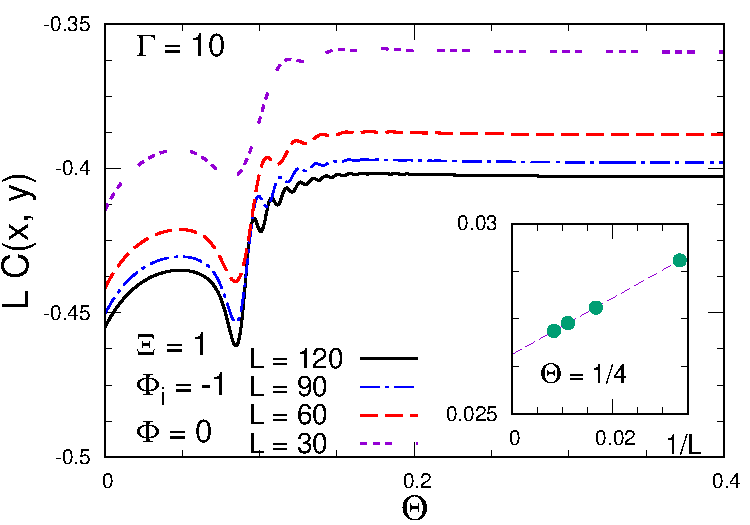
\includegraphics[width=0.45\columnwidth]{imm/LCk-1q0e100t100S10000.pdf}
      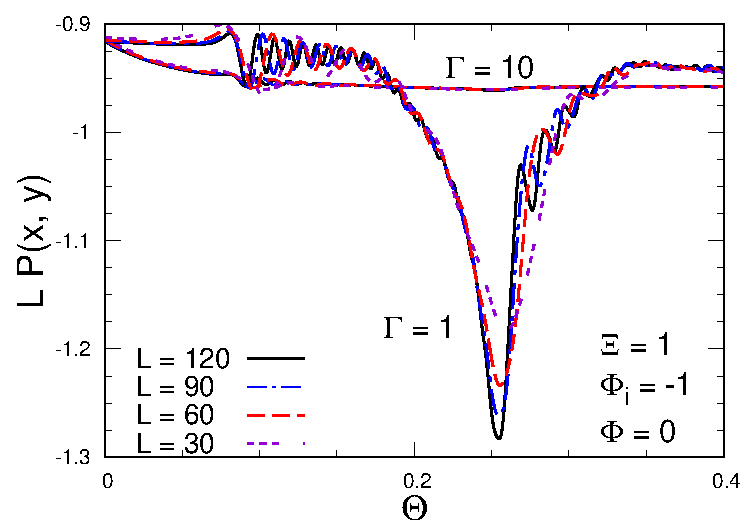
\includegraphics[width=0.45\columnwidth]{imm/LPk-1q0e100t100S10000.pdf}
        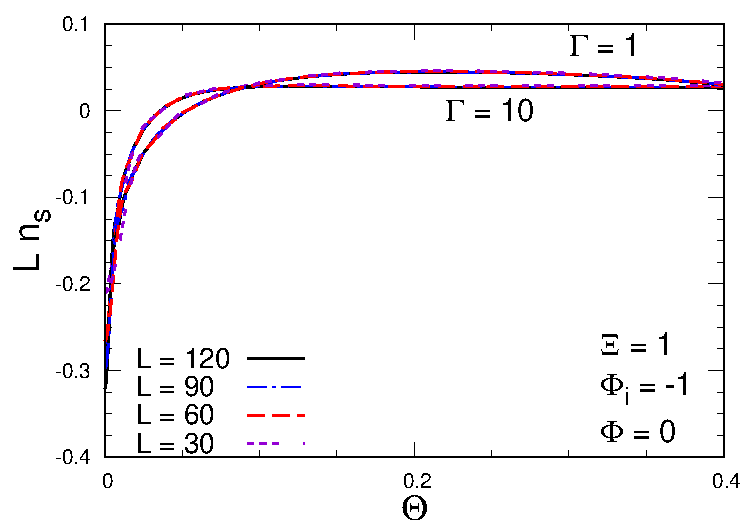
\includegraphics[width=0.45\columnwidth]{imm/LNk-1q0e100t100S10000.pdf}
        \caption{Quantum evolutions along the dissipative protocol, fully
          supporting the OFSS reported in Eqs.~(\ref{Oscaquefssprotb1})
          and (\ref{Oscaquefssprotb2}). We report curves for $L\,n_s$
          (bottom), $L\,P(x=L/3,y=2L/3,t)$ (middle), and
          $C(x=L/3,y=2L/3,t)$ (top), for various values of $L$, at fixed
          $\Phi_i=-1$, $\Phi=0$, $\Xi=1$, and two values of
          $\Gamma=L^z\gamma$, i.e.  $\Gamma=1,\,10$ (except for the top
          figure where we only report data for $\Gamma=10$ to ensure a
          good readability).  The inset of the top figure shows that the
          OFSS is approached with $O(1/L)$ corrections. Analogous results
          are obtained for other values of the scaling variables. }
      \label{protbresgammaresc}
\end{figure}

In conclusion, on the basis of the above scaling arguments, the OFSS
arising from the dissipative QQ protocols in the presence of a thermal
bath is expected to be given by
\begin{eqnarray}
   O_a(t, L, w_i, w, T, \gamma) \, \approx \, L^{-y_o} \,
  {\cal O}_a(\Theta, \Phi_i, \Phi, \Xi, \Gamma),\quad
  \label{Oscaquefssprotb1}
\end{eqnarray}
and
\begin{eqnarray}
&& G_{O}(t, {\bm x}_1, {\bm x}_2, L, w_i, w, T, \gamma)  \, \approx
    \label{Oscaquefssprotb2} \\
    &&\qquad\qquad
     L^{-2y_o} \, {\cal G}_{O}(\Theta, {\bm X}_1, {\bm X}_2, \Phi_i,
    \Phi, \Xi, \Gamma). \qquad \nonumber
\end{eqnarray}
In the large-$\Gamma$ limit the above OFFS behaviors at fixed $\Xi$ is
expected to approach the corresponding equilibrium FSS, faster and
faster in terms of $\Theta$, matching the behavior at finite $\gamma$.
Moreover, we also expect that the equilibrium FSS is also approached
in the large-$\Theta$ limit at fixed $\Gamma$ and $\Xi$, independently
of $\Gamma$, but faster and faster with increasing~$\Gamma$.

Again, the numerical results for the particle density $n_s(t)$ and
correlation functions $P$ and $C$ fully support the above OFSS
equations, i.e. Eq.~(\ref{Oscaquefssprotb1}) for $n_s(t)$ with
$y_o=y_n=1$, and Eq.~(\ref{Oscaquefssprotb2}) for $P$ and $C$ with
$y_o=y_c=1/2$. Some results are reported in
Fig.~\ref{protbresgammaresc}.  We also stress that analogous results
are expected for other observables, for example the correlation
functions of the spin operator of the equivalent formulation provided
by the quantum Ising chains.

